\begin{frame}[plain]
    \begin{bee}[Lernziele]
        \begin{enumerate}[1)]
            \item Die Definitionen "Künstliche Intelligenz", "Machine Learning" und "Deep Learning" können in eigenen Worten erläutert werden
            \item Die Unterteilungen "Supervised Learning", "Semi-Supervised Learning", "Unsupervised Learning", "Reinforcement Learning" sind ein Begriff
            \item Die Funktionsweise und Limitationen der linearen und logistischen Regression sind verstanden
            \item Die Funktionsweise des Rosenblatt Perzeptrons und deren Anwendung ist verstanden
            \item Das Grundpzinzip von Neuronalen Netzen ist verstanden und kann selbständig schematisch aufgezeichnet werden
            \item Generative KI und deren Anwendungen sind bekannt
            \item KI-Andwendungmöglichkeiten in der Medizin resp. Radiologie können anhand deren Impact, Herausforderungen, etc. eruiert werden

        \end{enumerate}
    \end{bee} 
\end{frame}

\begin{frame}{KI Definition}
    \begin{bee}[]
        \textbf{"Künstliche Intelligenz ist die Fähigkeit einer Maschine, menschliche Fähigkeiten wie logisches Denken, Lernen, Planen, and Kreativität zu imitieren."} \end{bee}
\end{frame}

\begin{frame}[plain]
    \begin{figure}[hp]
    \centering
    \captionsetup{font=footnotesize}
    
    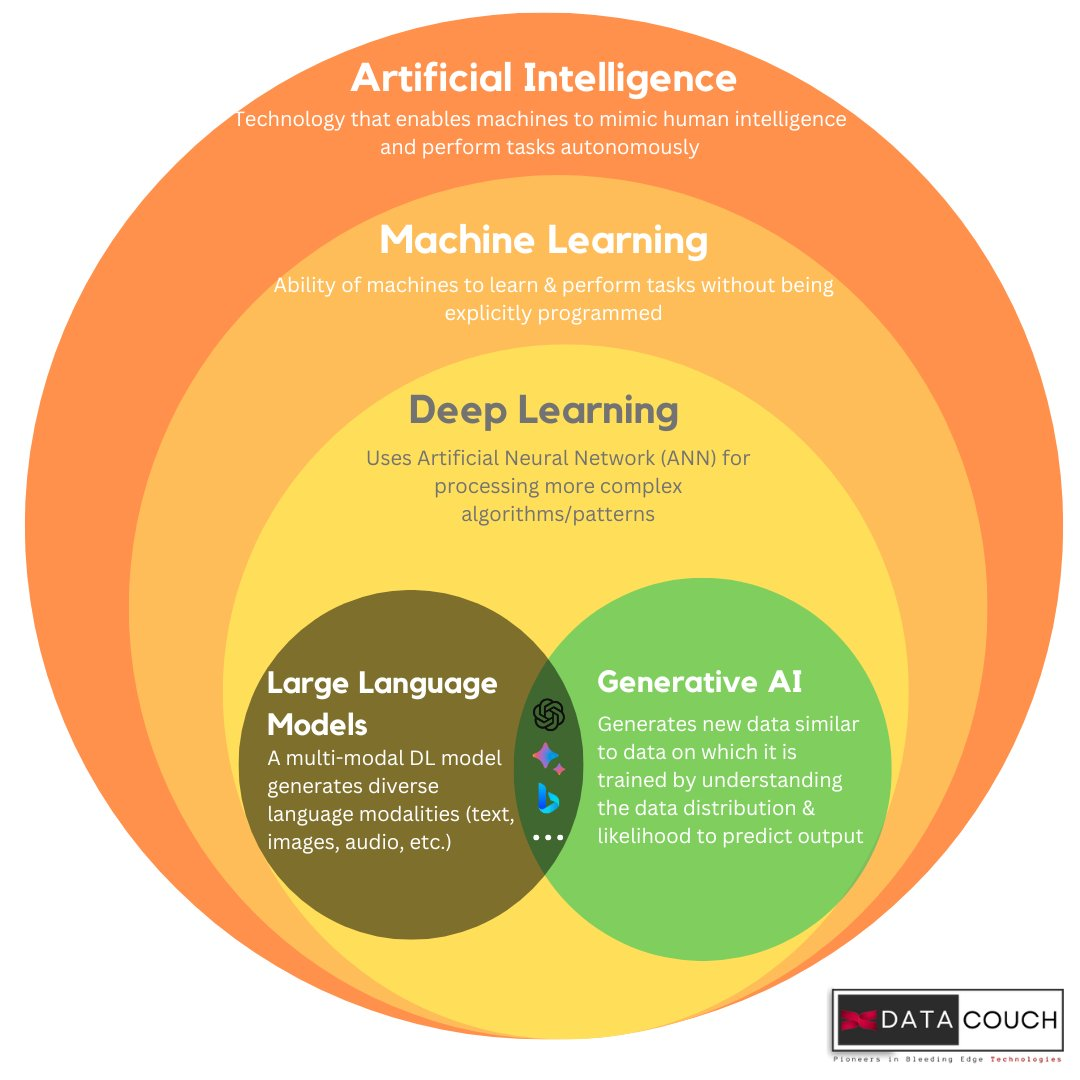
\includegraphics[scale=.21]{2-content/FyQhPzmakAErIJy.jpeg}
    
    \caption{\url{https://x.com/datacouch_io/status/1667494319916462080}}
    \end{figure}
\end{frame}

\begin{frame}{Die 4 KI Modelle}
    \begin{bee}
        \begin{enumerate}[$\bullet$]
            \item \textbf{Reaktive KI:} Produziert vorhersehbare Ergebnisse auf der Grundlage der Eingaben (Bsp.: Deep Blue)
            \item \textbf{KI mit begrenzter Speicherkapazität:} Selbständige Weiterentwicklung aufgrund bereits Erlerntem (Bsp.: Selbstfahrende Autos)
            \item \textbf{Theory of Mind:} Menschenähnliche Entscheidungsfähigkeiten
            \item \textbf{KI mit Selbsterkenntnis:} Eigene Emotionen und Zustände sowie der anderer Menschen bewusst
        \end{enumerate}
    \end{bee}
\end{frame}

\begin{frame}{KI History}
    \begin{bee}[Frühgeschichte]
        \begin{enumerate}[$\bullet$]
            \item Mensch ist fasziniert, eine nicht-menschliche Form der Intelligenz zu erschaffen
            \item Griechische Mythologie: Bronzeroboter namens Talos, der Kreta bewacht
            \item China: Maschinenbauingenieur konstruiert lebensgrossen Roboter, der nahezu menschlich erschien
        \end{enumerate}
    \end{bee}
\end{frame}

\begin{frame}{KI History II}
    \begin{bee}[Ab dem 17. Jahrhundert]
        \begin{enumerate}[$\bullet$]
            \item 17. Jh.: Maschinen, um grosse Zahlen schneller und zuverlässiger zu berechnen
            \item 1837: Charles Babbage designed die Allzweck Rechenmaschine “Analytical Engine”
            \item Ada Lovelace entwickelte den ersten Computeralgorithmus "Note G" zur Berechnung von Bernoulli Zahlen
            \item 1940er-Jahren erster digitaler Computer "Z3" von Konrad Zuse
           \item Mit dem digitalen Zeitalter beginnen auch die entscheidenten Fortschritte in der KI
        \end{enumerate}
    \end{bee}
\end{frame}

\begin{frame}[plain]{Allzweck Rechenmaschine “Analytical Engine”}
    \begin{figure}[hp]
    \centering
    \captionsetup{font=footnotesize}
    
    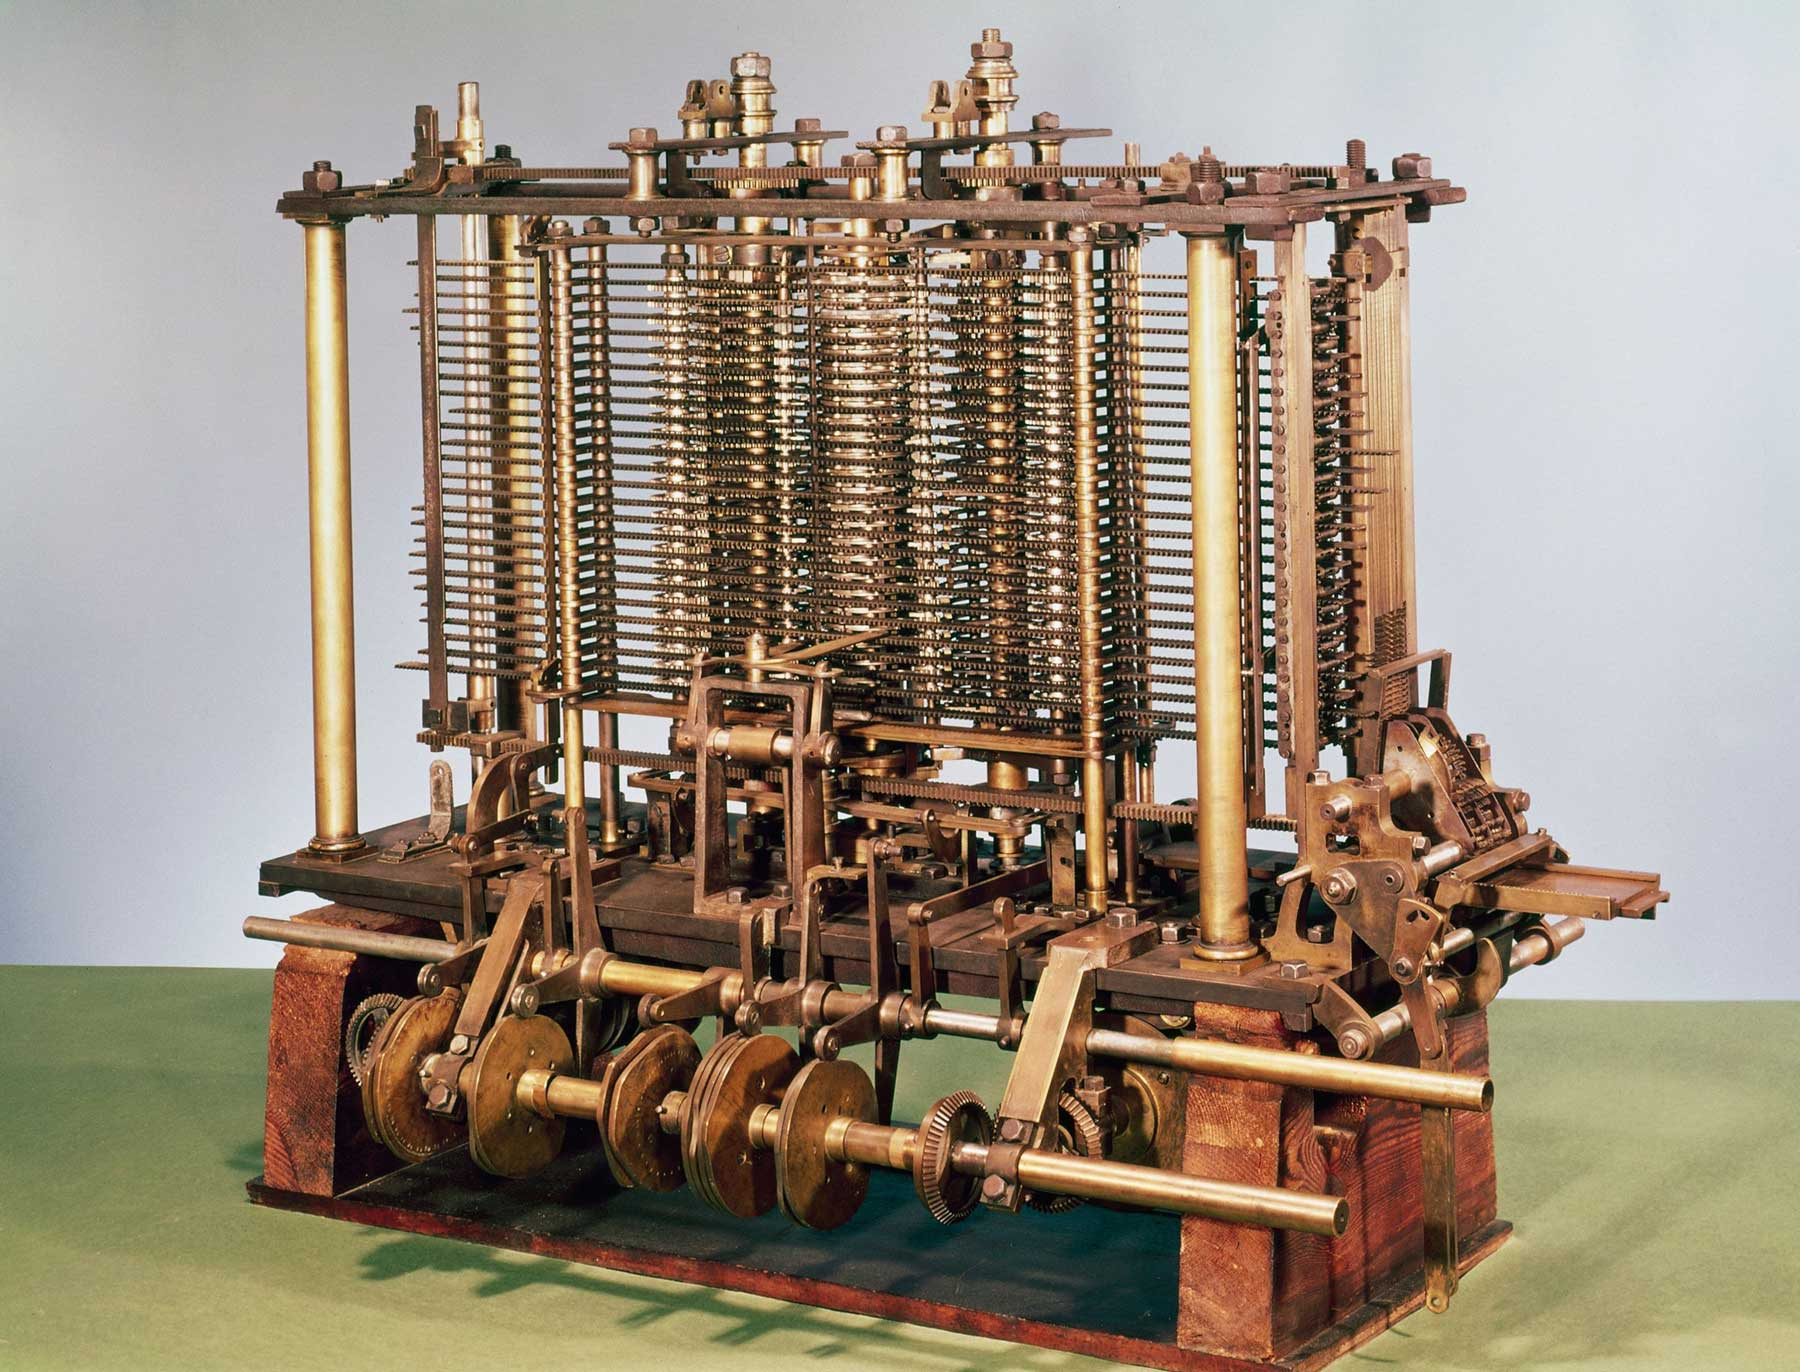
\includegraphics[scale=.14]{2-content/analytical-engine-1.jpg}
    
    \caption{\url{https://cronatec.ch/how-did-the-analytical-engine-work/}}
    \end{figure}
\end{frame}

\begin{frame}[plain]{Digitaler Computer “Z3“}
    \begin{figure}[hp]
    \centering
    \captionsetup{font=footnotesize}
    
    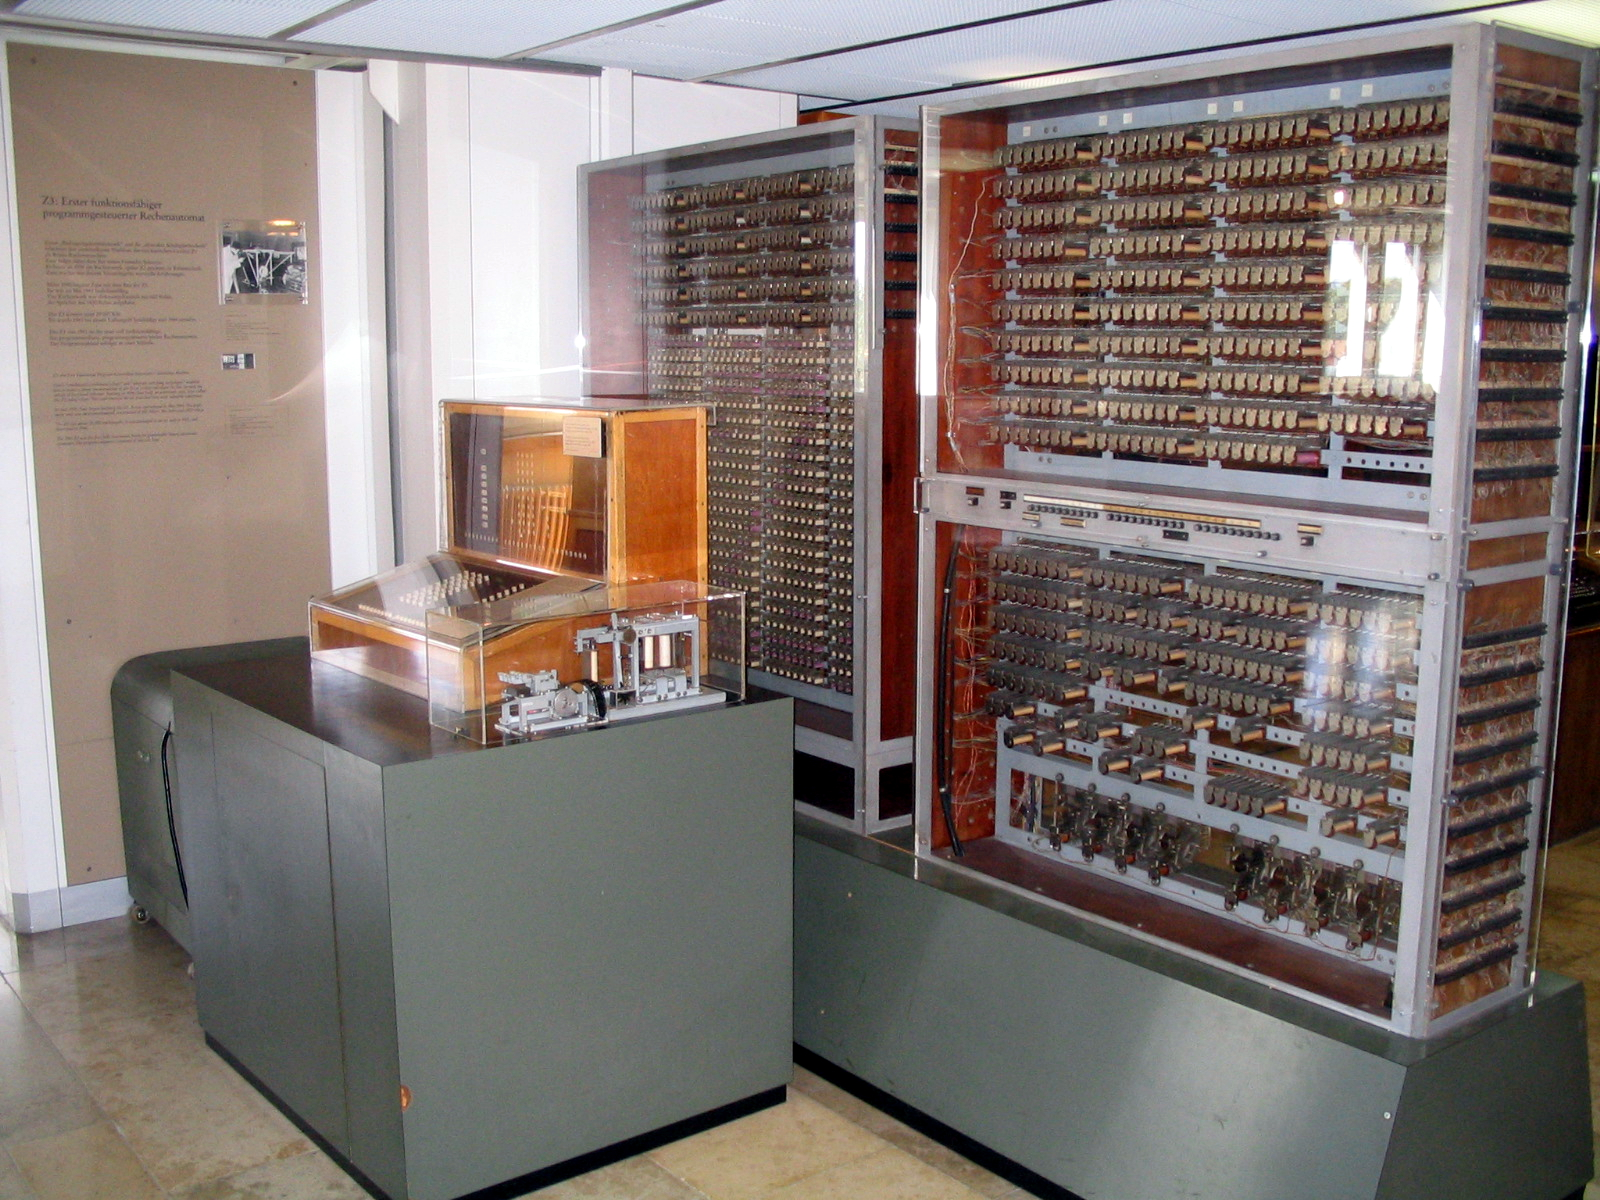
\includegraphics[scale=.4]{2-content/Z3_Deutsches_Museum.JPG}
    
    \caption{\url{https://cronatec.ch/how-did-the-analytical-engine-work/}}
    \end{figure}
\end{frame}

\begin{frame}{KI History III}
    \begin{bee}[Literatur und Film]
        \begin{enumerate}[$\bullet$]
            \item Drei Gesetze der Robotik im Roman "Ich, der Robot" von Isaac Asimov. Koexistenz von Menschen und autonomen Robotern
            \item 2001: Odyssee im Weltraum der Raumschiffcomputer HAL9000 von Stanley Kubrick
            \item Marvel Universe: J.A.R.V.I.S (Just A Rather Very Intelligent System)
        \end{enumerate}
    \end{bee}
\end{frame}

\begin{frame}{KI History IV}
    \begin{bee}[Ab 1950]
        \begin{enumerate}[$\bullet$]
            \item Vision: Rechner können mehr als programmierte Befehle ausführen
        \end{enumerate}
    \end{bee}
\end{frame}

\begin{frame}[plain]
    \begin{figure}[hp]
    \centering
    \captionsetup{font=footnotesize}
    
    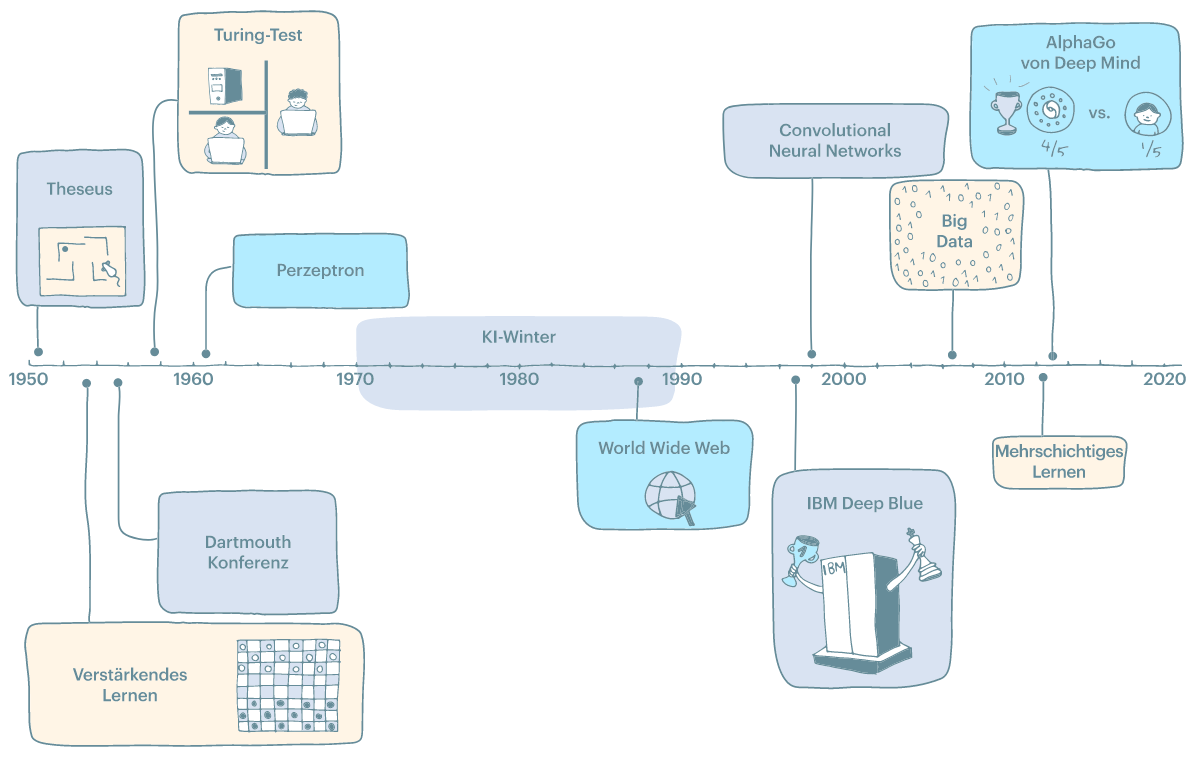
\includegraphics[scale=.3]{2-content/KI_History.png}
    
    \caption{\url{https://www.thats-ai.org/de-CH/units/eine-kurze-geschichte-der-ki}}
    \end{figure}
\end{frame}

\begin{frame}[plain]
    \begin{figure}[hp]
    \centering
    \captionsetup{font=footnotesize}
    
    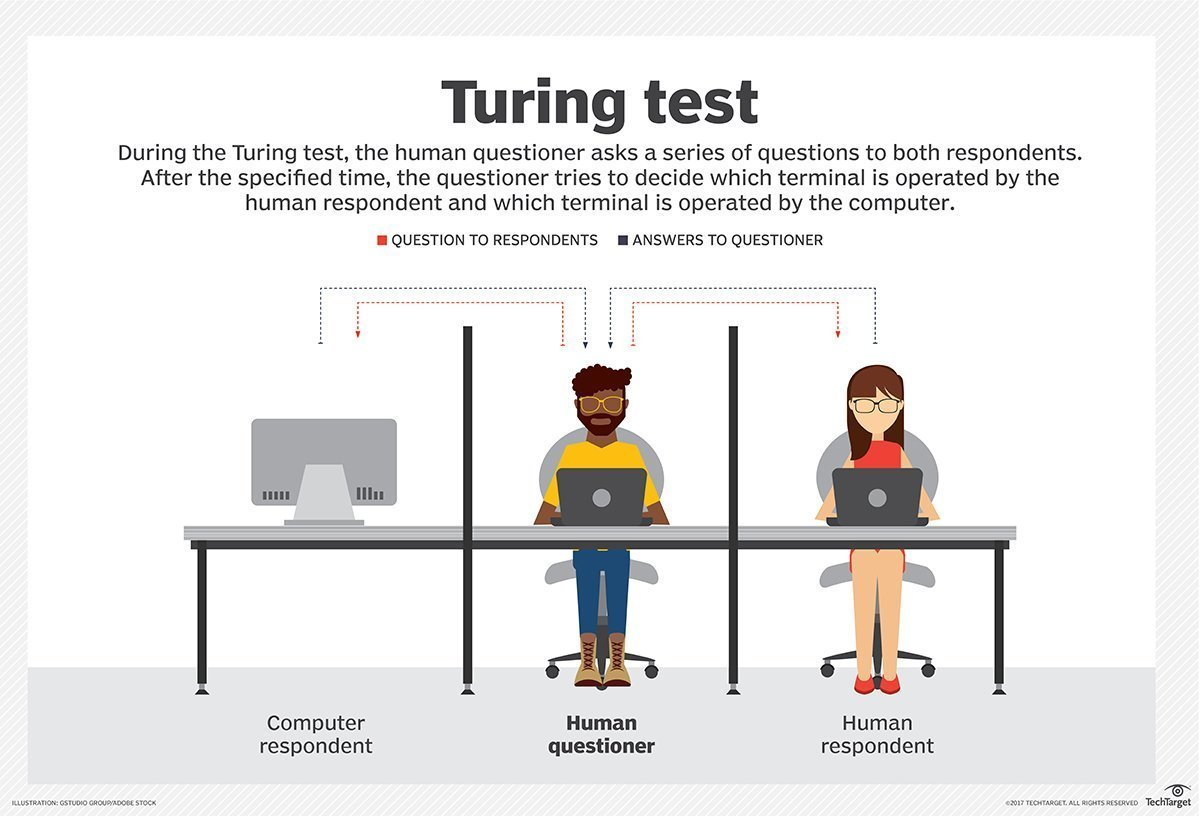
\includegraphics[scale=.27]{2-content/crm-turing_test.jpg}
    
    \caption{\url{https://www.techtarget.com/searchenterpriseai/definition/Turing-test}}
    \end{figure}
\end{frame}

\begin{frame}[plain]{KI Entwicklung - Key Drivers I}
    \begin{columns}
        \begin{column}{4cm}
           \begin{bee}[Big Data]
             Zunahme Verfügbarkeit von Daten aus verschiedenen Quellen
            \end{bee}
    
        \end{column}
        \begin{column}{4cm}
                \begin{bee}[Technologischer Fortschritt]
                Anzahl Transistoren im Computer verdoppeln sich alle 2 Jahre (Moore's Law). Geringere Speicherkosten und mehr Rechenpower
            \end{bee}
        \end{column}
    \end{columns}
\end{frame}

\begin{frame}[plain]{KI Entwicklung - Key Drivers II}
    \begin{columns}
        \begin{column}{4cm}
          \begin{bee}[Awareness]
                Awareness Geschäftsprozesse zu optimieren, Kosten zu senken und neue Einnahmequellen zu erschließen
            \end{bee}
        \end{column}
        \begin{column}{4cm}
            \begin{bee}[Algorithmen]
               Verbesserten Algorithmen ermöglichen es, komplexe Probleme zu lösen, die früher als unlösbar galten
            \end{bee}
        \end{column}
    \end{columns}
\end{frame}

\begin{frame}[plain]
    \begin{figure}[hp]
    \centering
    \captionsetup{font=scriptsize}
    
    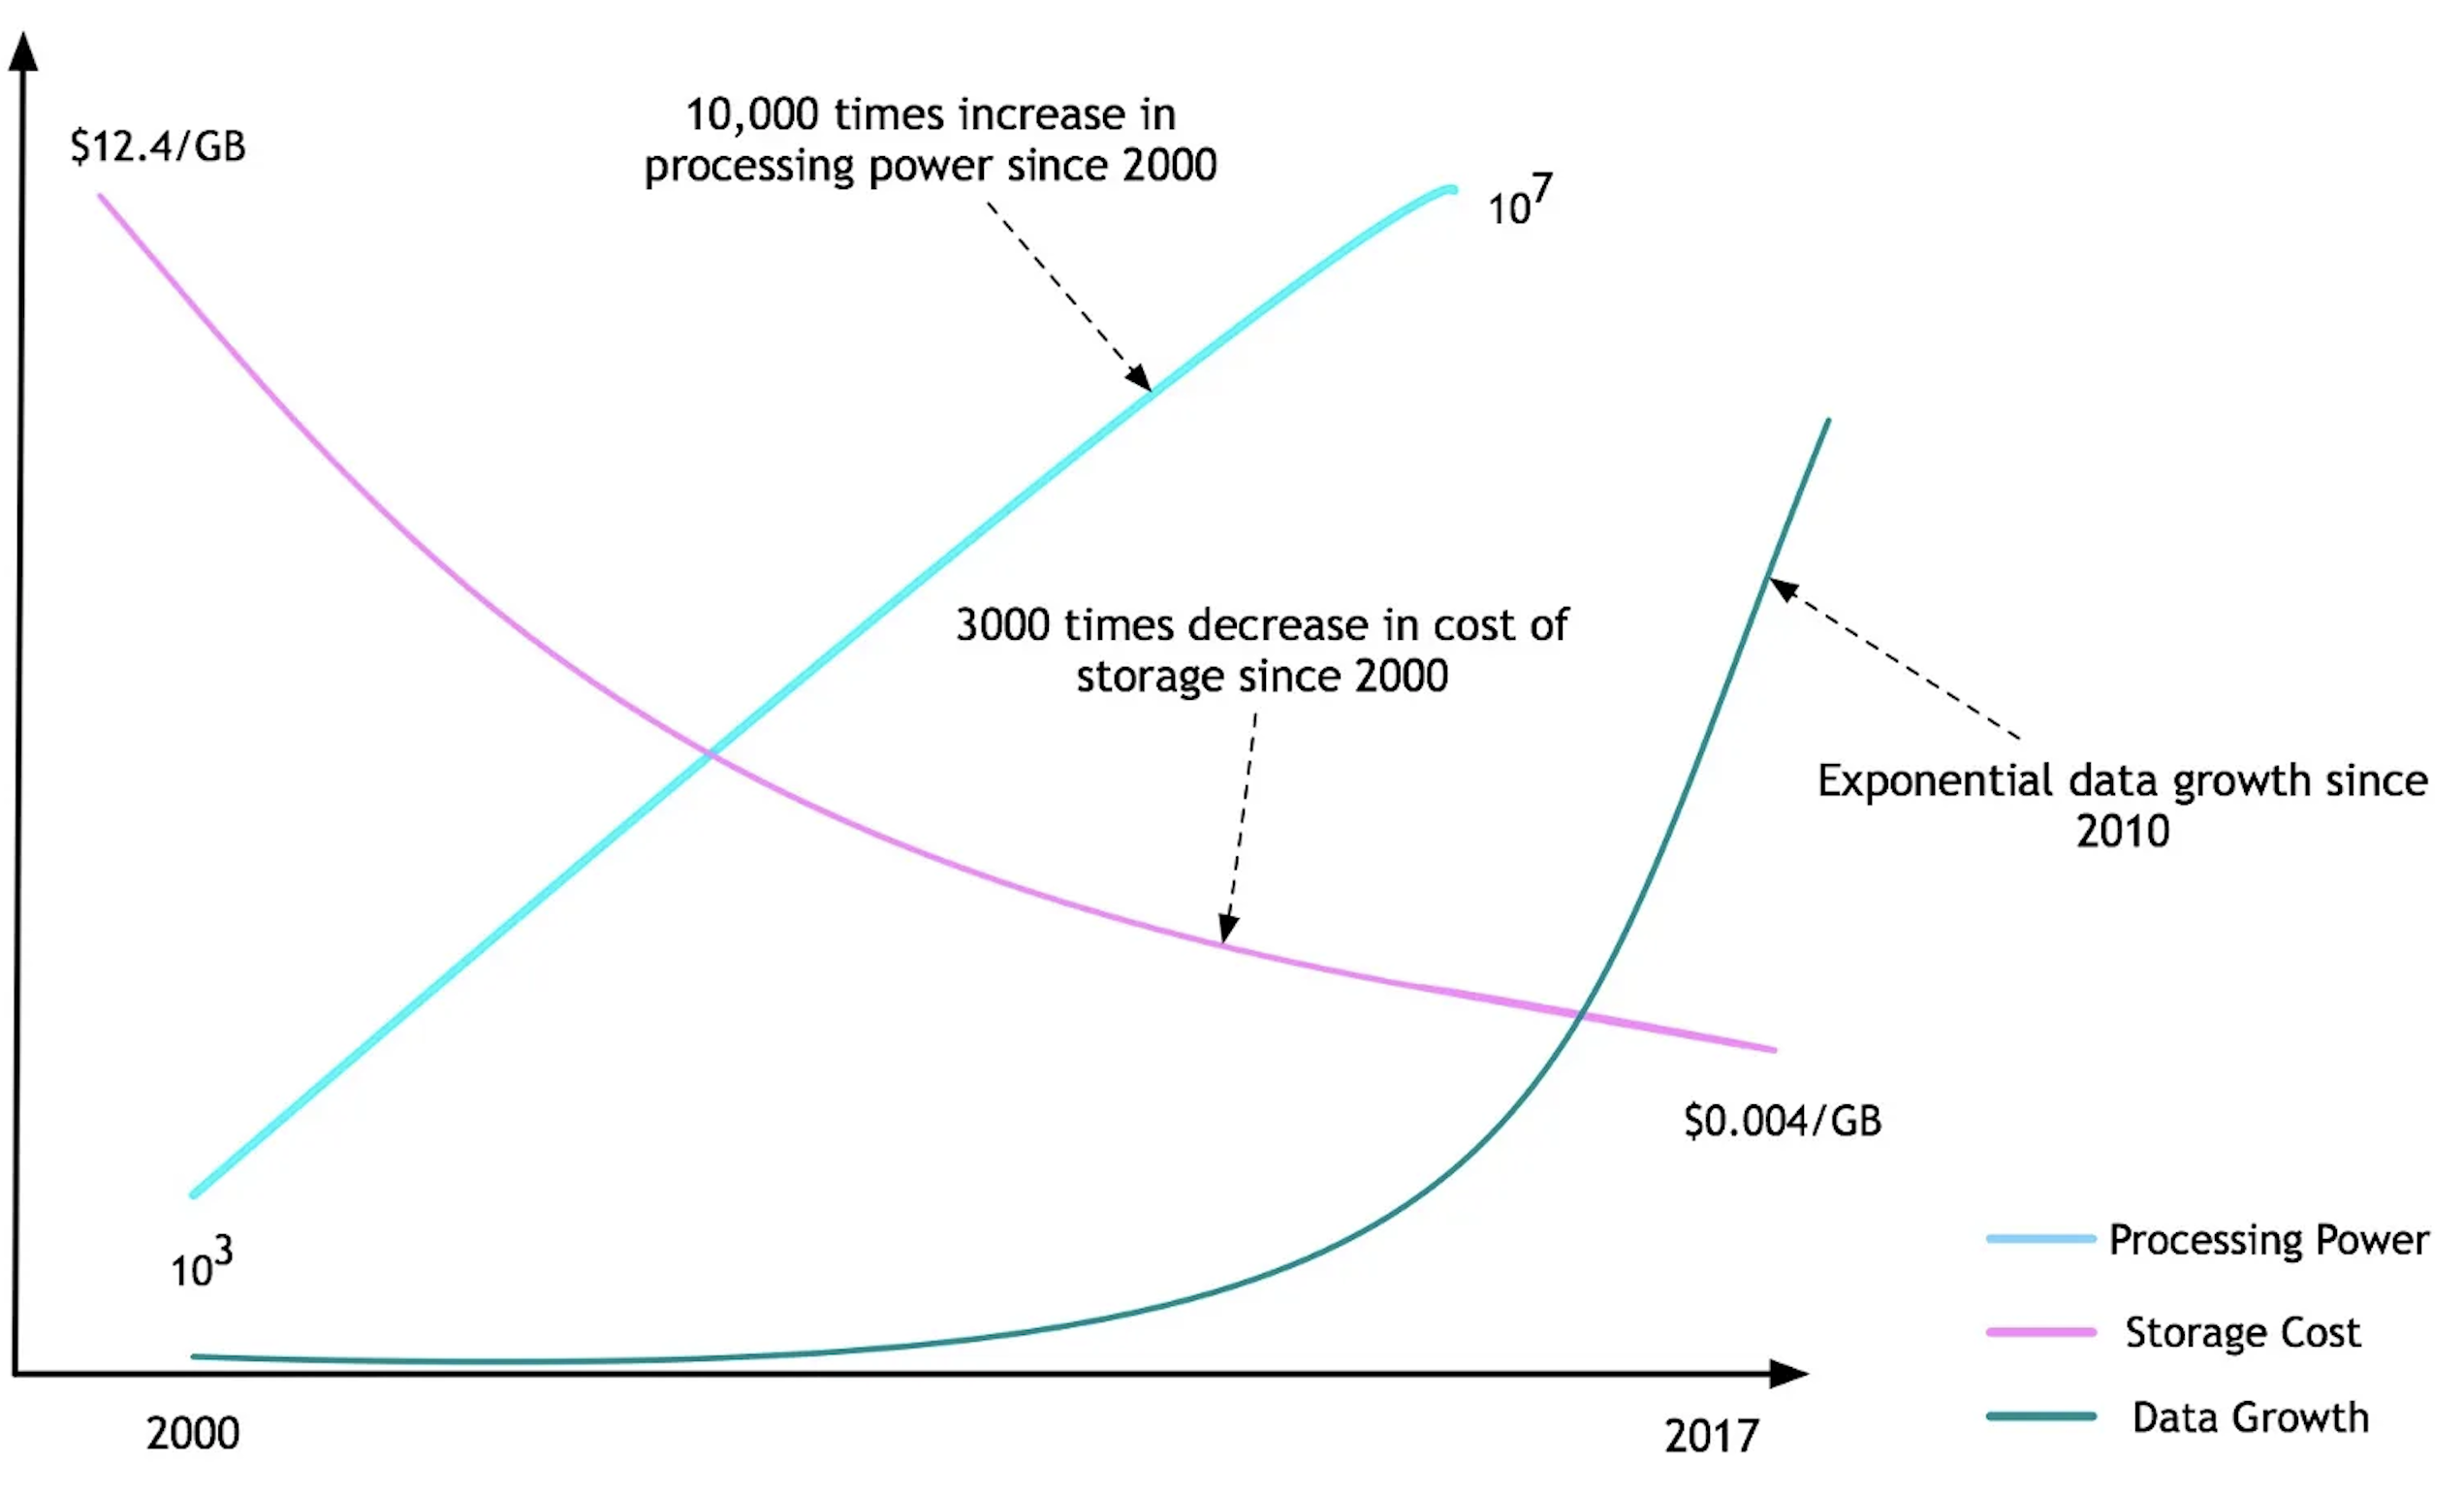
\includegraphics[scale=.28]{2-content/moores_law.png}
    
    \caption{\url{https://towardsdatascience.com/the-future-of-computation-for-machine-learning-and-data-science-fad7062bc27d}}
    \end{figure}
\end{frame}

\begin{frame}[plain]
    \begin{figure}[hp]
    \centering
    \captionsetup{font=scriptsize}
    
    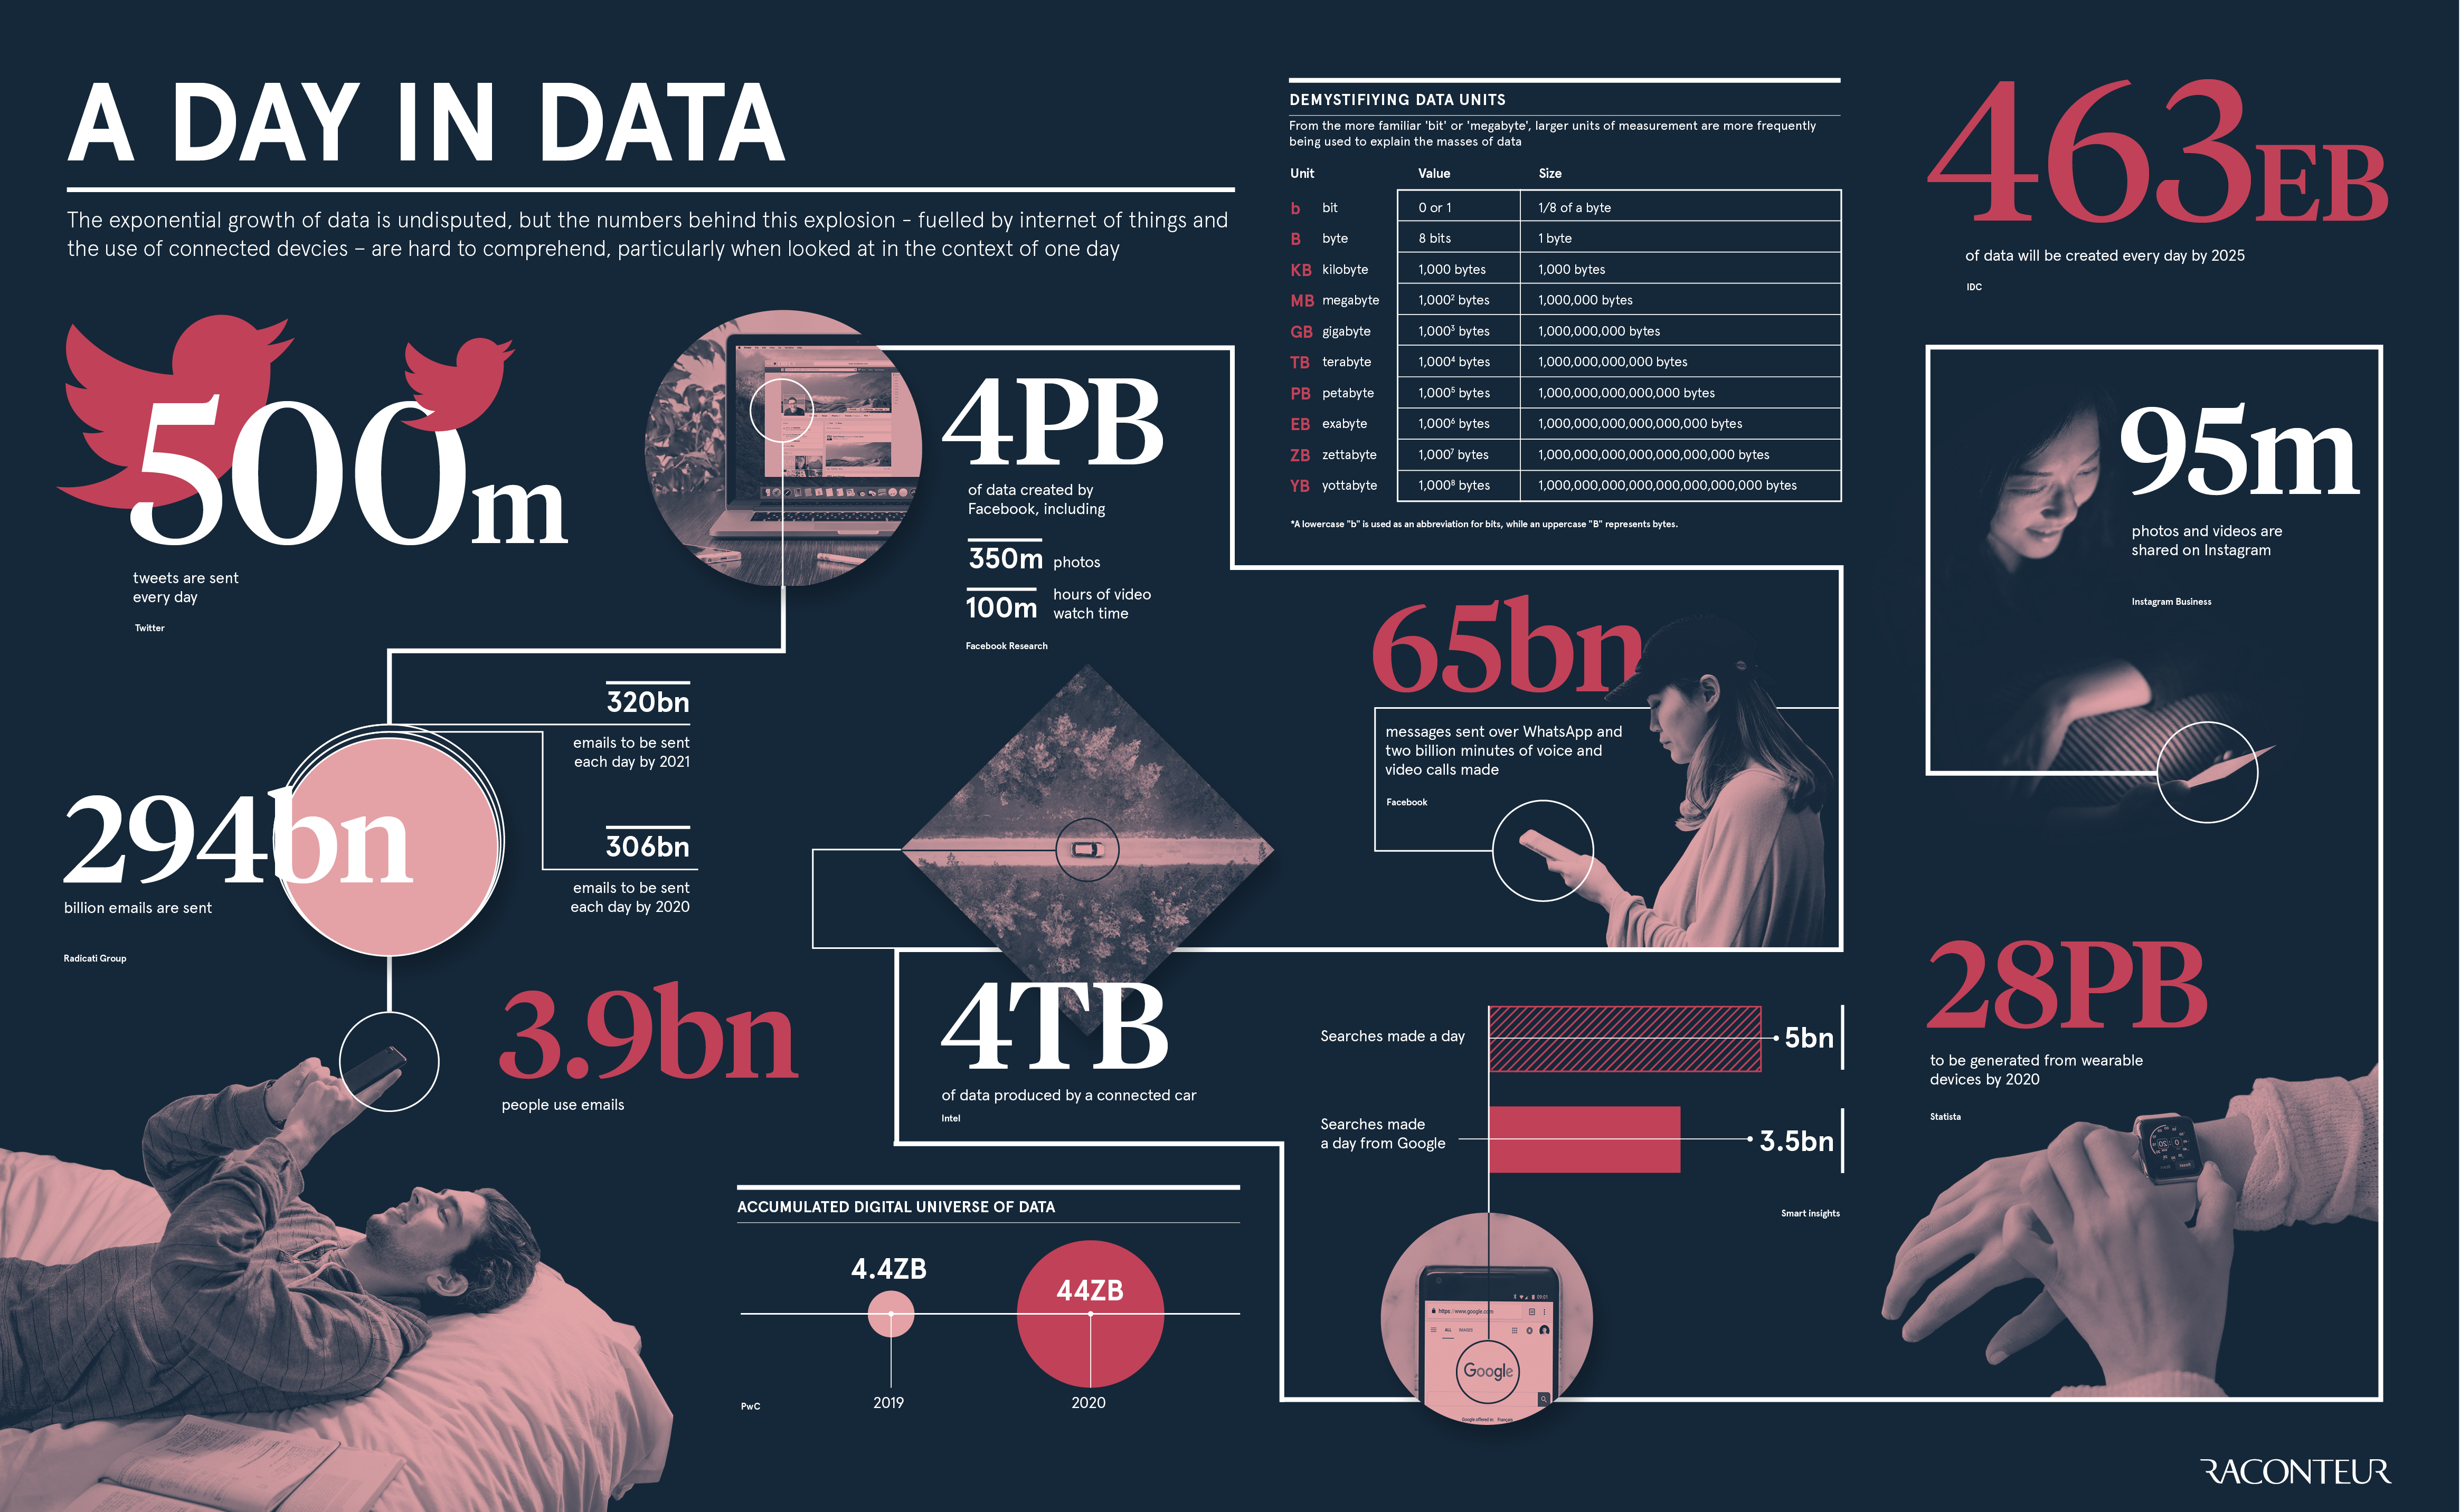
\includegraphics[scale=.072]{2-content/data_generation.jpg}
    
    \caption{\url{https://www.weforum.org/agenda/2019/04/how-much-data-is-generated-each-day-cf4bddf29f/}}
    \end{figure}
\end{frame}

\begin{frame}[plain]
    \begin{figure}[hp]
    \centering
    \captionsetup{font=scriptsize}
    
    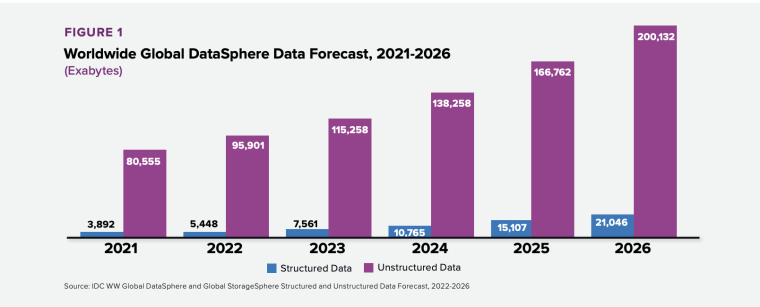
\includegraphics[scale=.70]{2-content/data_generation2.png}
    
    \caption{\url{https://www.business2community.com/statistics-pages/how-much-data-is-created-every-day}}
    \end{figure}
\end{frame}

\begin{frame}[plain]
    \begingroup
        \fontfamily{qag}\selectfont
        \Huge\color{black}\textbf{Machine Learning}\\[0.6em]
    \endgroup
    \begingroup
    \endgroup
\end{frame}

\begin{frame}[plain]
    \begin{figure}[hp]
    \centering
    \captionsetup{font=scriptsize}
    
    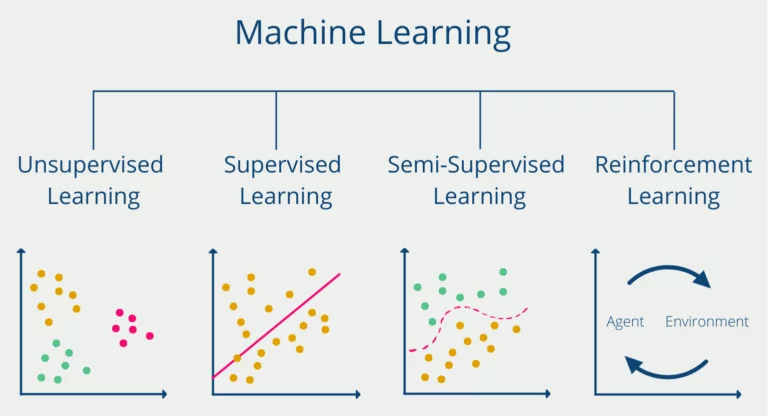
\includegraphics[scale=.5]{2-content/ml_fields.png}
    
    \caption{\url{https://databasecamp.de/ki/unsupervised-learning}}
    \end{figure}
\end{frame}

\begin{frame}{Unsupervised Learning}
    \begin{bee}[Einsatzgebiete]
        \begin{enumerate}[$\bullet$]
            \item Recommender Systems
            \item Anomaly detection
            \item Customer Segmentation
            \item ...
        \end{enumerate}
    \end{bee}
\end{frame}

\begin{frame}{Unsupervised Learning}
    \begin{bee}[Algorithmen]
        \begin{enumerate}[$\bullet$]
            \item k-Means Clustering
            \item DBSCAN
            \item Autoencoders
            \item ...
        \end{enumerate}
    \end{bee}
\end{frame}

\begin{frame}[plain]{k-Means Clustering}
    \begin{figure}[Algorithmen]
    \centering
    \captionsetup{font=scriptsize}
    
    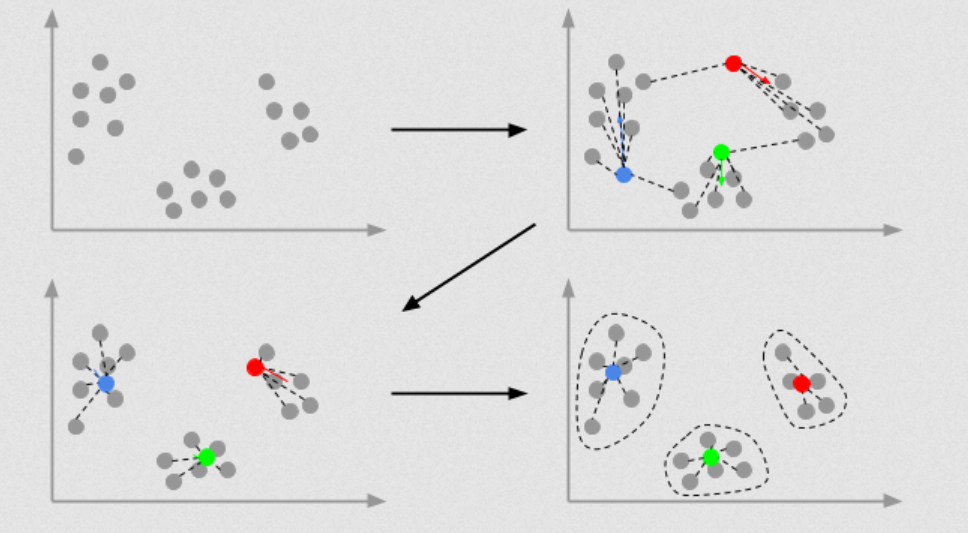
\includegraphics[scale=.35]{2-content/Screenshot from 2024-06-10 23-13-00.png}
    
    \caption{\url{https://www.davidthol.com/clustering-mit-hilfe-des-k-means-algorithmus/}}
    \end{figure}
\end{frame}

\begin{frame}[plain]{Clustering - DBSCAN vs k-Means}
    \begin{figure}[Algorithmen]
    \centering
    \captionsetup{font=scriptsize}
    
    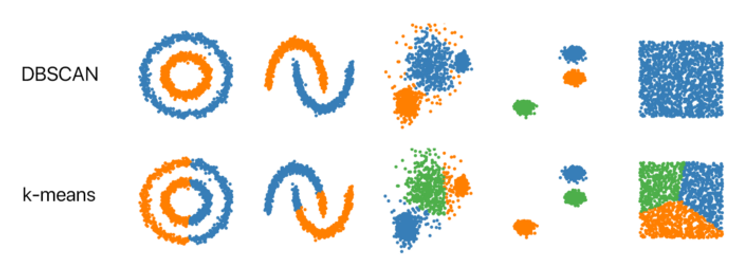
\includegraphics[scale=.5]{2-content/3eee0b_79f8969aef9e47edb2f6169e57c0dc55~mv2.png}
    
    \caption{\url{https://www.theaidream.com/post/dbscan-clustering-algorithm-in-machine-learning}}
    \end{figure}
\end{frame}

\begin{frame}[plain]{Supervised Learning}
    \begin{figure}[hp]
    \centering
    \captionsetup{font=scriptsize}
    
    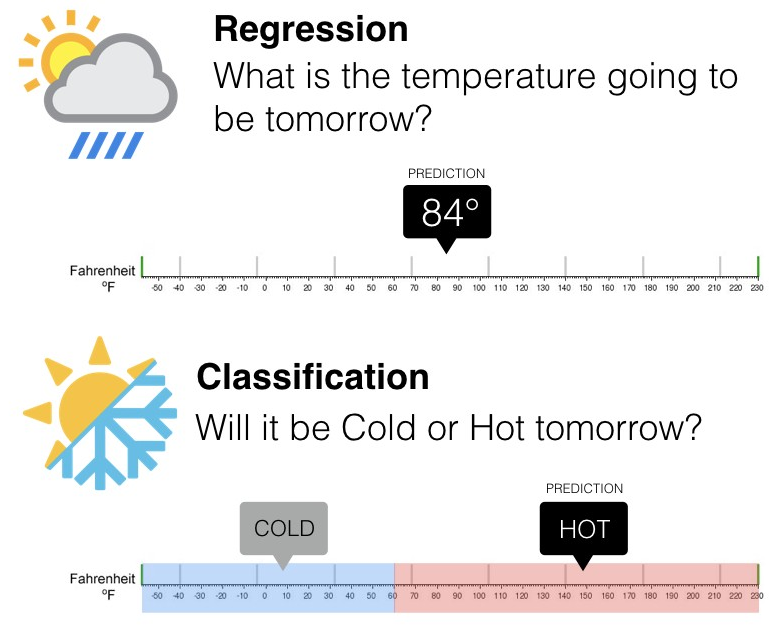
\includegraphics[scale=.3]{2-content/regression-vs.-classification.png}
    
    \caption{\url{https://www.springboard.com/blog/data-science/regression-vs-classification/}}
    \end{figure}
\end{frame}

\begin{frame}[plain]{Lineare Regression}
    \begin{figure}[hp]
    \centering
    \captionsetup{font=scriptsize}
    
    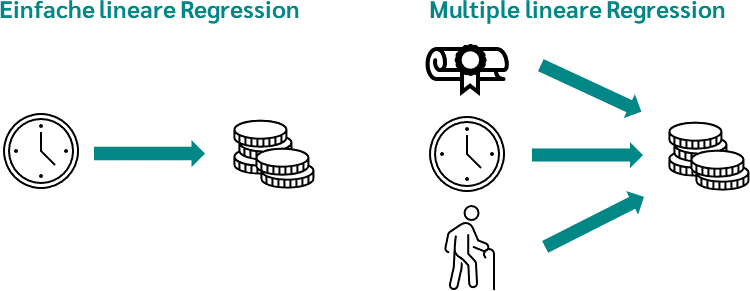
\includegraphics[scale=.6]{2-content/Lineare_Regression.png}
    
    \caption{\url{https://www.springboard.com/blog/data-science/regression-vs-classification/}}
    \end{figure}
\end{frame}

\begin{frame}[plain]{Lineare Regression - Beispiel}
    \begin{figure}[hp]
    \centering
    \captionsetup{font=scriptsize}
    
    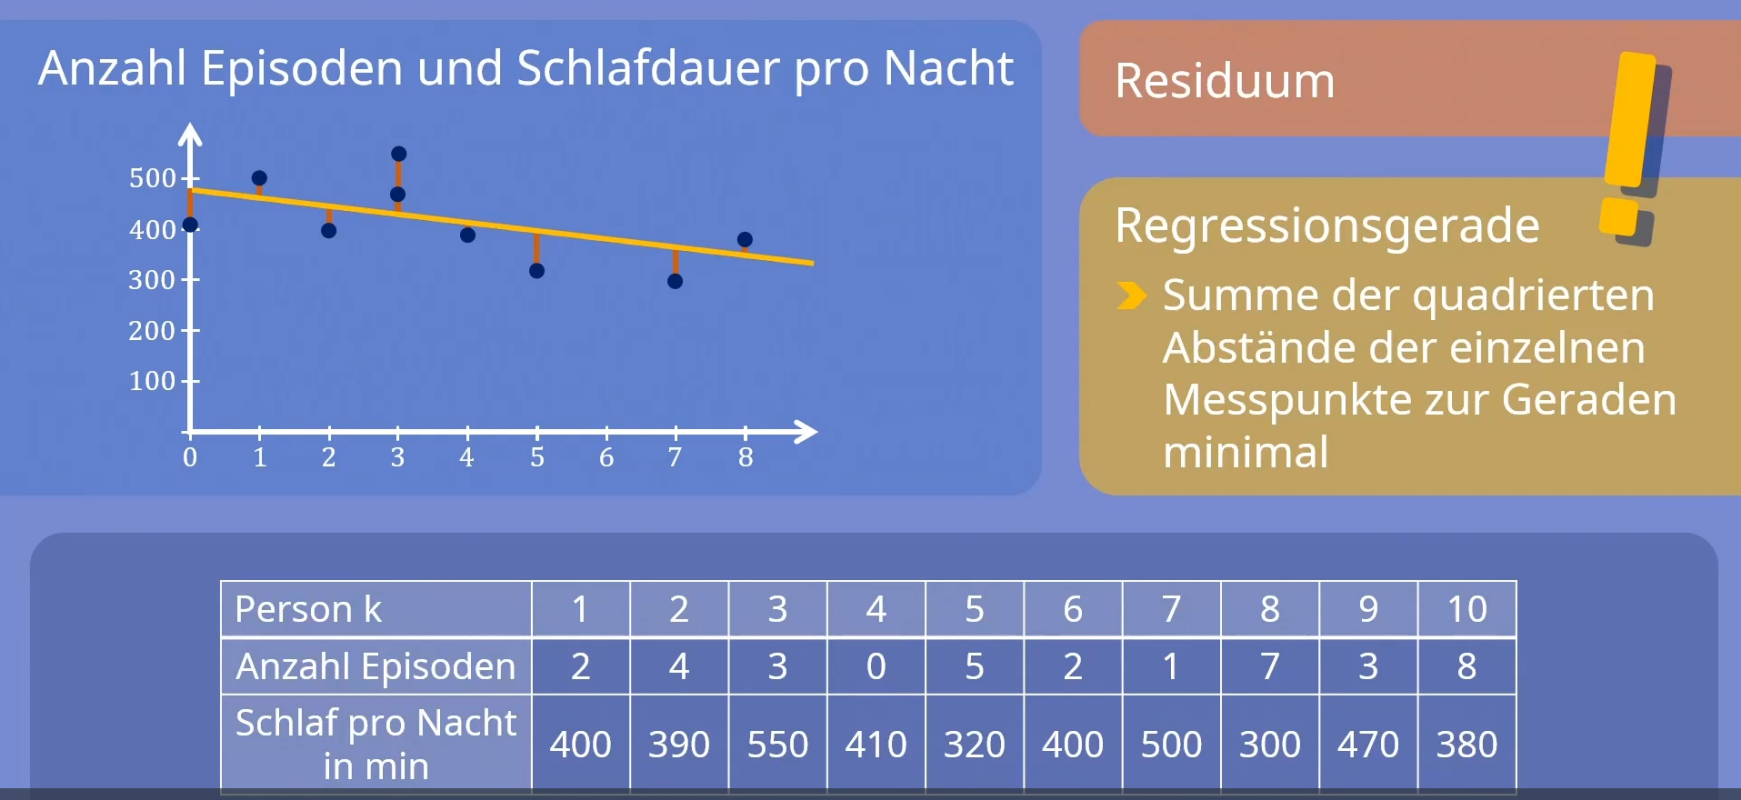
\includegraphics[scale=.23]{2-content/Lin_reg_example.png}
    
    \caption{\url{https://studyflix.de/statistik/lineare-regression-2147}}
    \end{figure}
\end{frame}

\begin{frame}[plain]{Lineare Regression - Gleichung}
    \begin{figure}[hp]
    \centering
    \captionsetup{font=scriptsize}
    
    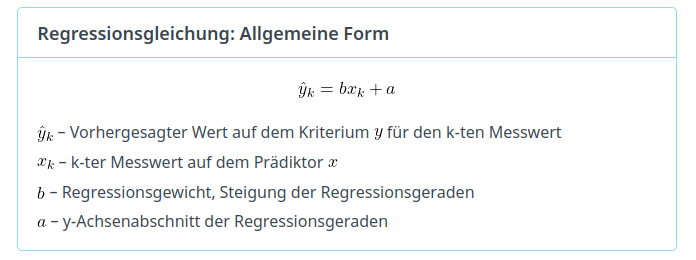
\includegraphics[scale=.5]{2-content/Lin_reg_formula.png}
    
    \caption{\url{https://studyflix.de/statistik/lineare-regression-2147}}
    \end{figure}
\end{frame}

\begin{frame}[plain]{Logistische Regression - Beispiel}
    \begin{figure}[hp]
    \centering
    \captionsetup{font=scriptsize}
    
    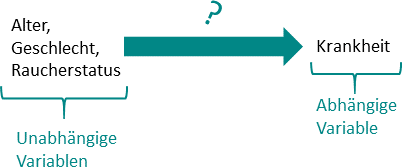
\includegraphics[scale=.9]{2-content/logistische-regression-beispiel.png}
    
    \caption{\url{https://datatab.de/tutorial/logistische-regression}}
    \end{figure}
\end{frame}

\begin{frame}[plain]{Logistische Regression - Beispiel II}
    \begin{figure}[hp]
    \centering
    \captionsetup{font=scriptsize}
    
    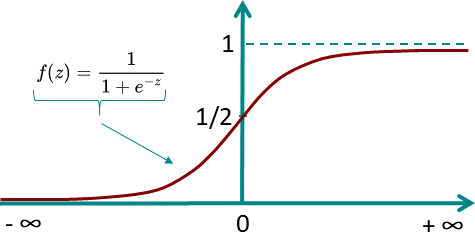
\includegraphics[scale=.8]{2-content/Logistische-Funktion.png}
    
    \caption{\url{https://datatab.de/tutorial/logistische-regression}}
    \end{figure}
\end{frame}

\begin{frame}[plain]
    \begingroup
        \fontfamily{qag}\selectfont
        \Huge\color{black}\textbf{Neuronale Netzwerke}\\[0.6em]
    \endgroup
    \begingroup
    \endgroup
\end{frame}

\begin{frame}[plain]{Beispiel aus der Digitaltechnik}
    \begin{figure}[hp]
    \centering
    \captionsetup{font=scriptsize}
    
    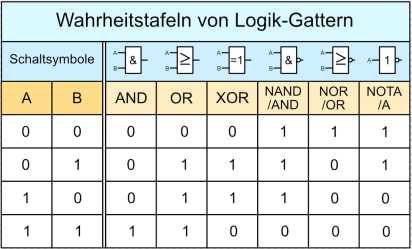
\includegraphics[scale=.8]{2-content/cache_18145092.png}
    
    \caption{\url{https://www.rahner-edu.de/grundlagen/signale-richtig-verstehen/digitaltechnik-teil-0/}}
    \end{figure}
\end{frame}

\begin{frame}[plain]{Einlagiges Perzeptron (1958)}
    \begin{figure}[hp]
    \centering
    \captionsetup{font=scriptsize}
    
    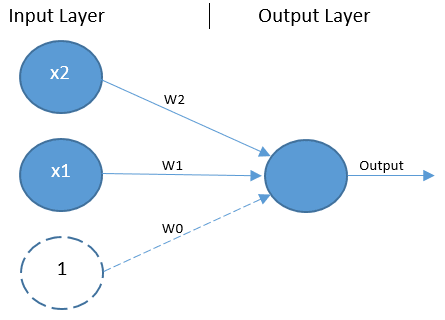
\includegraphics[scale=.6]{2-content/0 wOYoifz24Wz_I152.png}
    
    \caption{\url{https://dev.to/jbahire/demystifying-the-xor-problem-1blk}}
    \end{figure}
\end{frame}

\begin{frame}[plain]{Einlagiges Perzeptron (1958)}
    \begin{bee}[Algorithmus]
            \begin{enumerate}[1)]
                \item Multipliziere alle Inputs (xi) mit den entsprechenden Gewichten (wi)
                \item Summiere alle Resultate
                \item Aktiviere den Output (Threshold, Funktion)
                \item Vergleiche den Output mit dem erwarteten Wert und korrigiere die Gewichte entsprechend
            \end{enumerate}
    \end{bee} 
\end{frame}

\begin{frame}[plain]{Aktivierungsfunktion}
    \begin{figure}[hp]
    \centering
    \captionsetup{font=scriptsize}
    
    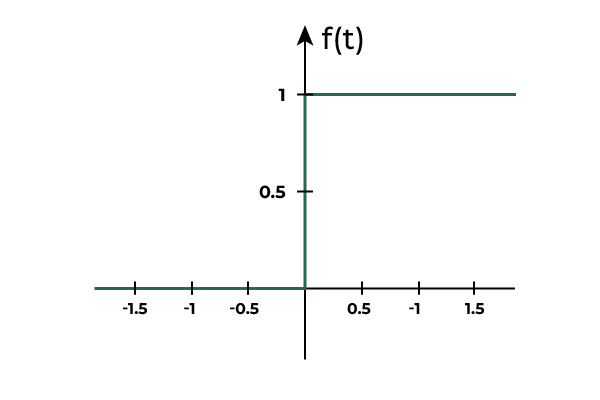
\includegraphics[scale=.5]{2-content/Stair-Step-function-03.png}
    
    \caption{\url{https://www.geeksforgeeks.org/stair-step-function/}}
    \end{figure}
\end{frame}

\begin{frame}[plain]{Einlagiges Perzeptron (1958) - Beispiel}
    \begin{bee}[Aufgabe]
        Ein AND-Gatter kann mit den folgenden Gewichten modelliert werden:
        \[ w_0=-1, w_1=1, w_2=1 \] 
            \begin{enumerate}[1)]
                \item Verifiziere, ob die Outputs wirklich dem AND-Gatter entsprechen
                \item Versuche, ob das Netzwerk für das OR-Gatter die entsprechenden Outputs generiert.
                \item Müssen evtl. die Gewichte angepasst werden? Versuche die Gewichte bei gleich bleibendem Bias zu ermitteln. \[ w_0=-1 \]
            \end{enumerate}
    \end{bee} 
\end{frame}

\begin{frame}[plain]{Klassifikation - XOR-Problem}
    \begin{figure}[hp]
    \centering
    \captionsetup{font=scriptsize}
    
    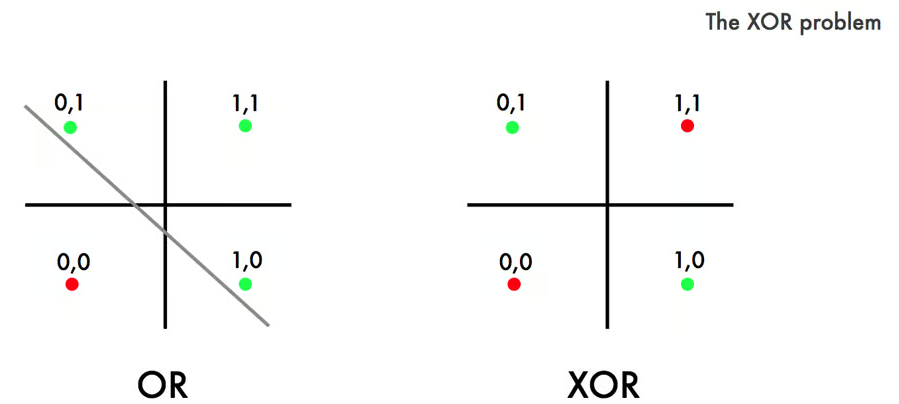
\includegraphics[scale=.4]{2-content/XOR.png}
    
    \caption{\url{https://dev.to/jbahire/demystifying-the-xor-problem-1blk}}
    \end{figure}
\end{frame}

\begin{frame}[plain]{Mehrlagiges Perzeptron}
    \begin{figure}[hp]
    \centering
    \captionsetup{font=scriptsize}
    
    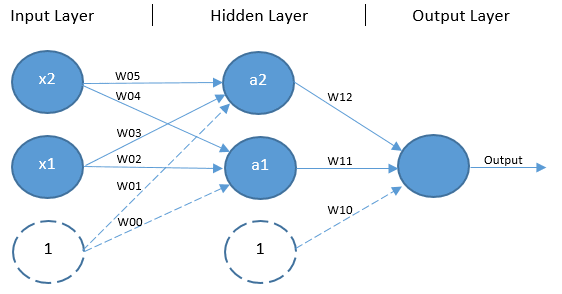
\includegraphics[scale=.6]{2-content/0 158hcRQzzw_wpEZW.png}
    
    \caption{\url{https://dev.to/jbahire/demystifying-the-xor-problem-1blk}}
    \end{figure}
\end{frame}

\begin{frame}[plain]{Backpropagation}
    \begin{figure}[hp]
    \centering
    \captionsetup{font=scriptsize}
    
    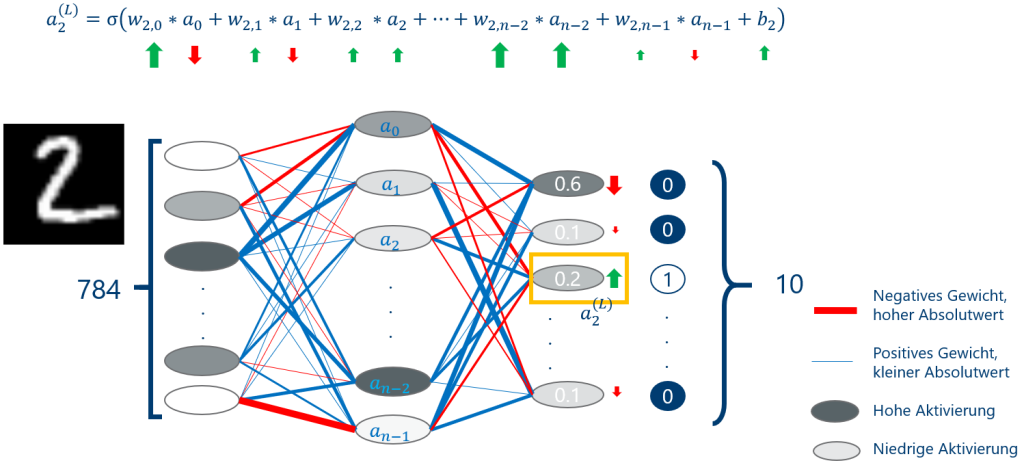
\includegraphics[scale=.5]{2-content/Graphic_Gradient-1024x463.png}
    
    \caption{\url{https://www.methodpark.de/blog/backpropagation-fuer-dummies/}}
    \end{figure}
\end{frame}

\begin{frame}[plain]{Convolutional Neural Network (CNN)}
    \begin{figure}[hp]
    \centering
    \captionsetup{font=scriptsize}
    
    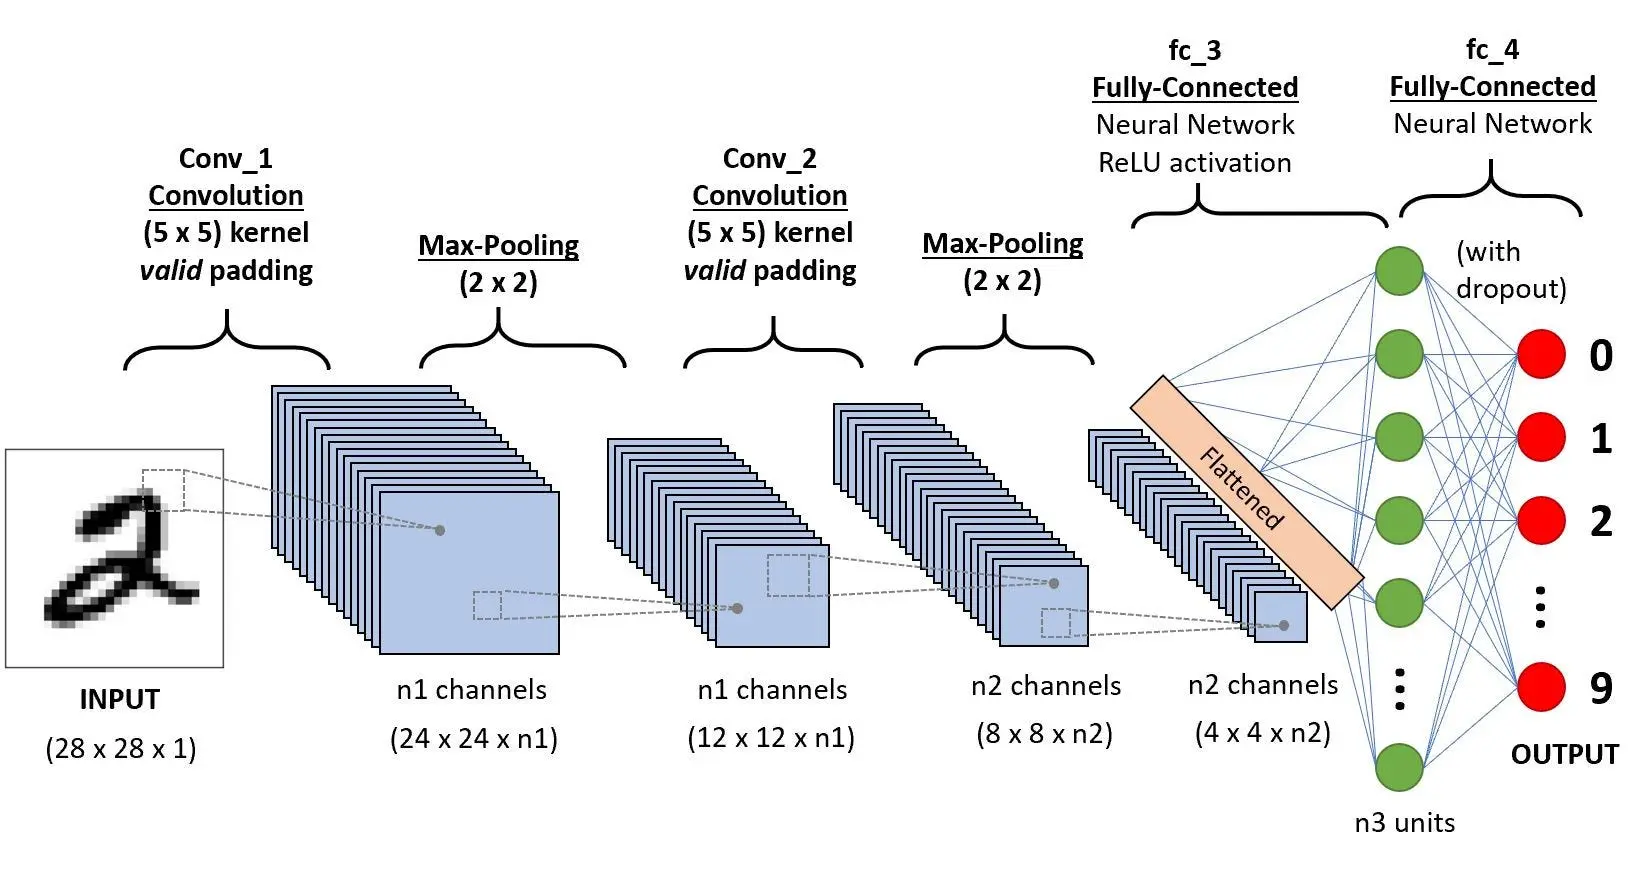
\includegraphics[scale=.22]{2-content/a-cnn-sequence-to-classify-handwritten-digits.png}
    
    \caption{\url{https://saturncloud.io/blog/}}
    \end{figure}
\end{frame}

\begin{frame}[plain]{CNN - Convolutional Layer}
    \begin{figure}[hp]
    \centering
    \captionsetup{font=scriptsize}
    
    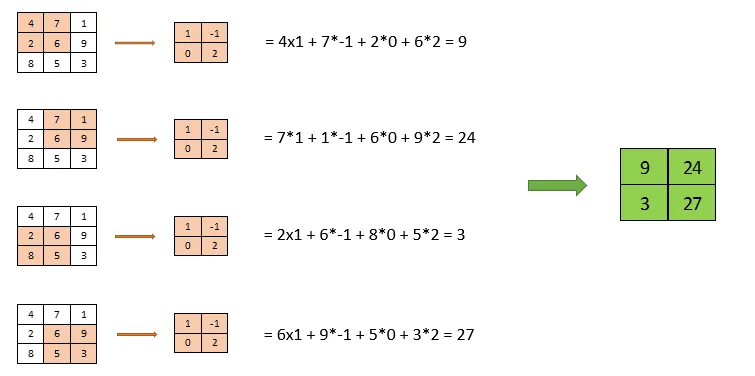
\includegraphics[scale=.5]{2-content/1_xrIgEHjLjwoonMMG-E5LxQ.png}
    
    \caption{\url{https://medium.com/@prajeeshprathap/}}
    \end{figure}
\end{frame}

\begin{frame}[plain]{CNN - Feature Maps}
    \begin{figure}[hp]
    \centering
    \captionsetup{font=scriptsize}
    
    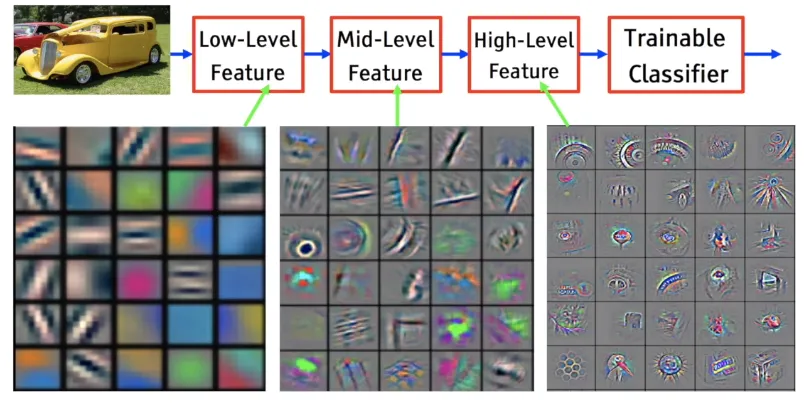
\includegraphics[scale=.5]{2-content/Feature_maps.png}
    
    \caption{\url{https://medium.com/analytics-vidhya/the-world-through-the-eyes-of-cnn-5a52c034dbeb}}
    \end{figure}
\end{frame}

\begin{frame}[plain]{Bias Variance Trade-Off I}
    \begin{figure}[hp]
    \centering
    \captionsetup{font=scriptsize}
    
    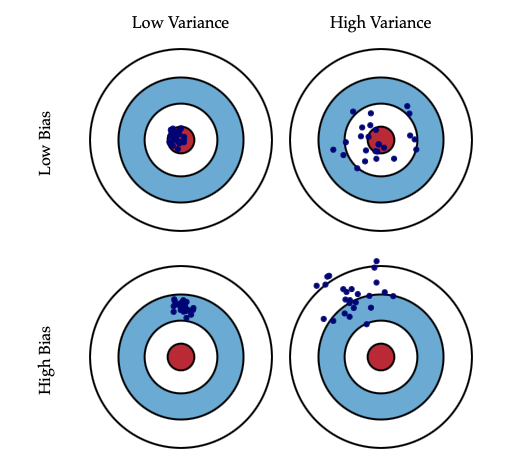
\includegraphics[scale=.4]{2-content/Screenshot 2024-06-11 at 13.06.13.png}
    
    \caption{\url{https://scott.fortmann-roe.com/docs/BiasVariance.html}}
    \end{figure}
\end{frame}

\begin{frame}[plain]{Bias Variance Trade-Off II}
    \begin{figure}[hp]
    \centering
    \captionsetup{font=scriptsize}
    
    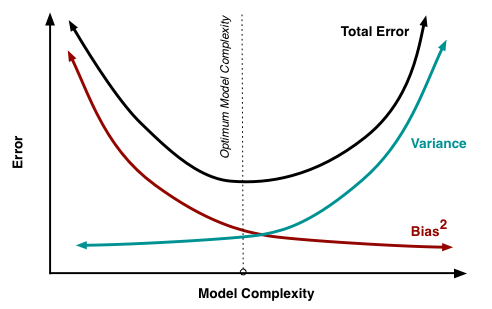
\includegraphics[scale=.6]{2-content/biasvariance.png}
    
    \caption{\url{https://scott.fortmann-roe.com/docs/BiasVariance.html}}
    \end{figure}
\end{frame}

\begin{frame}[plain]{Diskriminative vs. Generative}
    \begin{figure}[hp]
    \centering
    \captionsetup{font=footnotesize}
    
    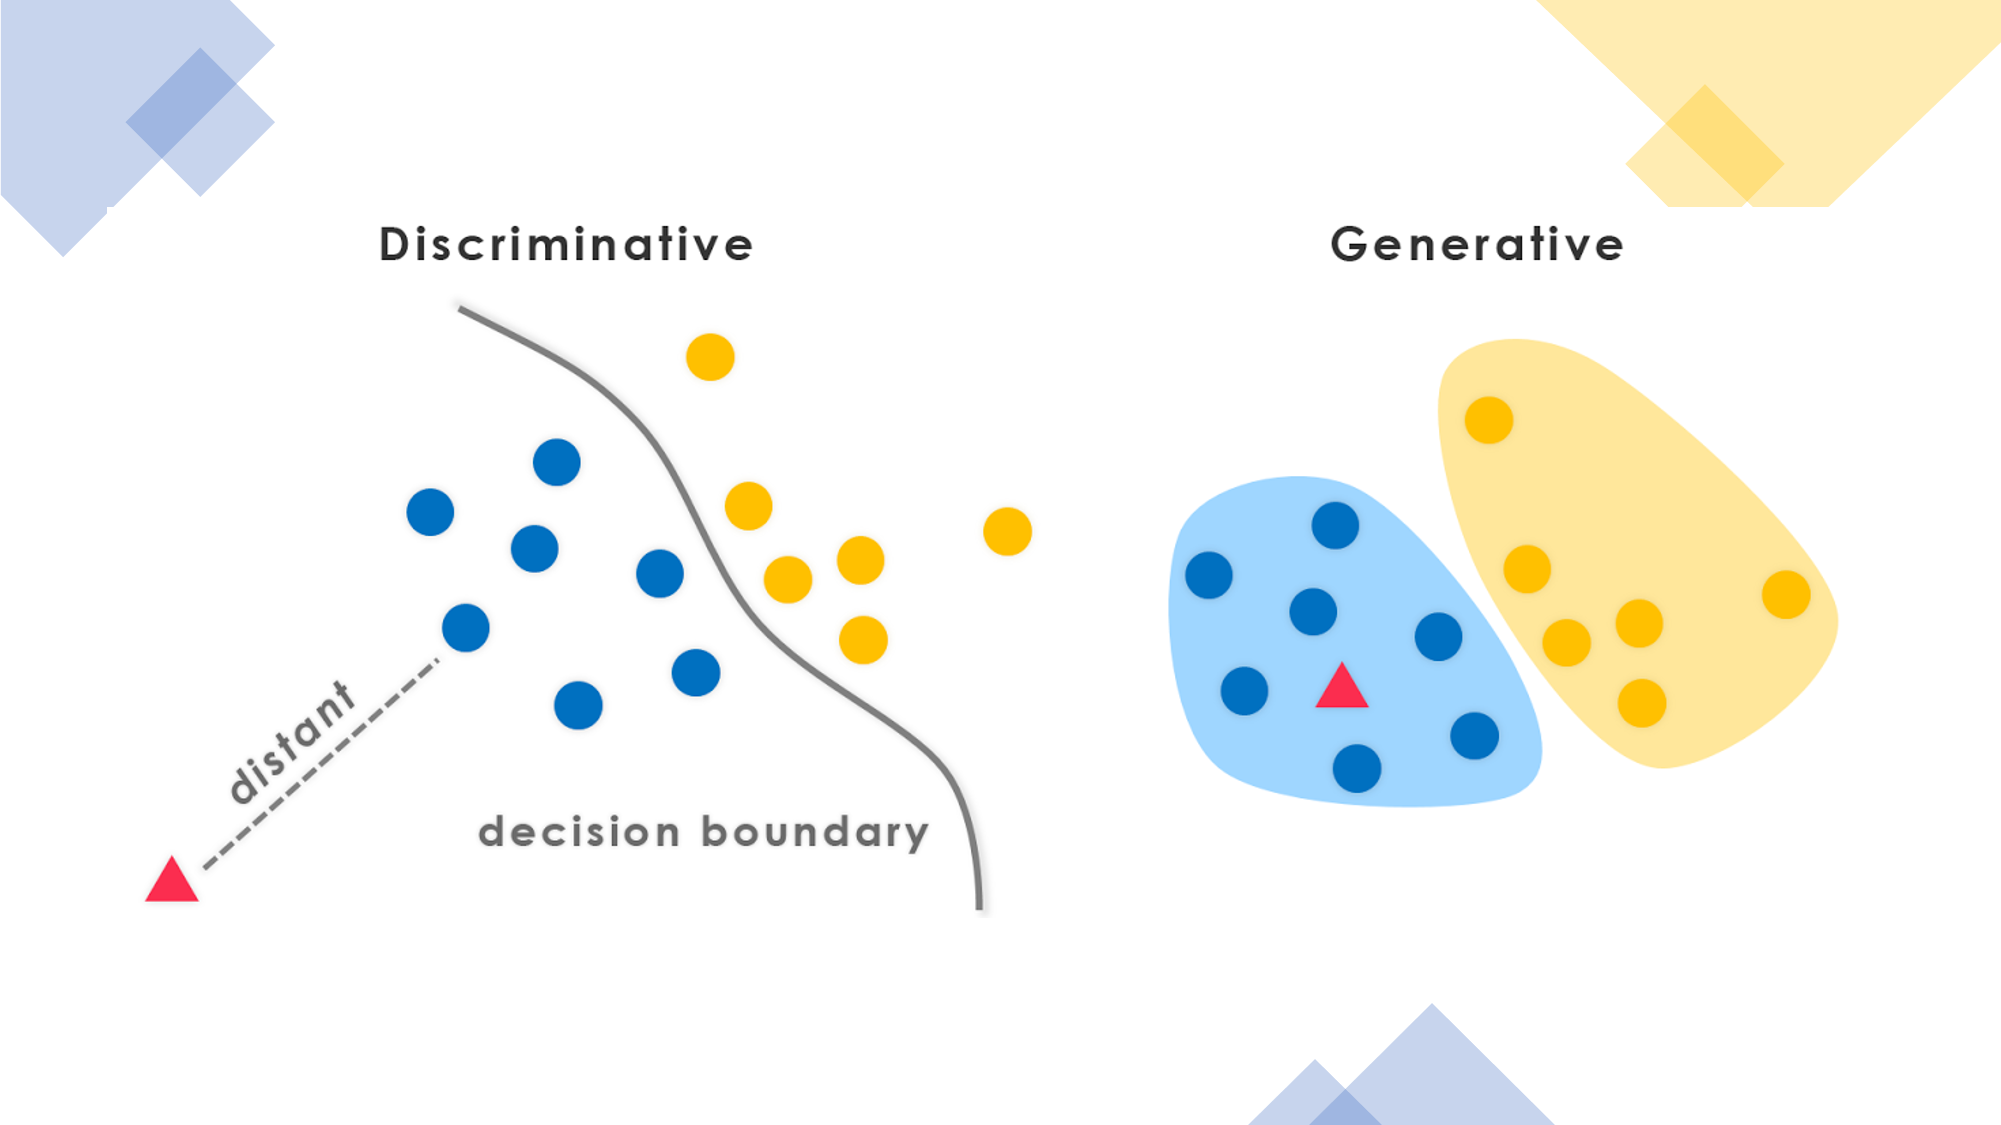
\includegraphics[scale=.15]{2-content/discriminative_generative.png}
    
    \caption{\url{https://www.kdnuggets.com/2020/05/microsoft-research-three-efforts-advance-deep-generative-models.html}}
    \end{figure}
\end{frame}

\begin{frame}[plain]{Chat-GPT}
    \begin{figure}[hp]
    \centering
    \captionsetup{font=footnotesize}
    
    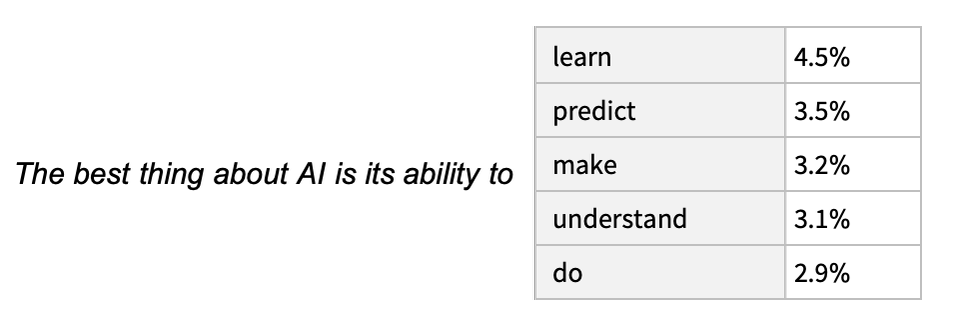
\includegraphics[scale=.7]{2-content/Screenshot 2024-06-11 at 23.05.31.png}
    
    \caption{\url{https://writings.stephenwolfram.com/2023/02/}}
    \end{figure}
\end{frame}

\begin{frame}[plain]{Chat-GPT Parameter Size}
    \begin{figure}[hp]
    \centering
    \captionsetup{font=footnotesize}
    
    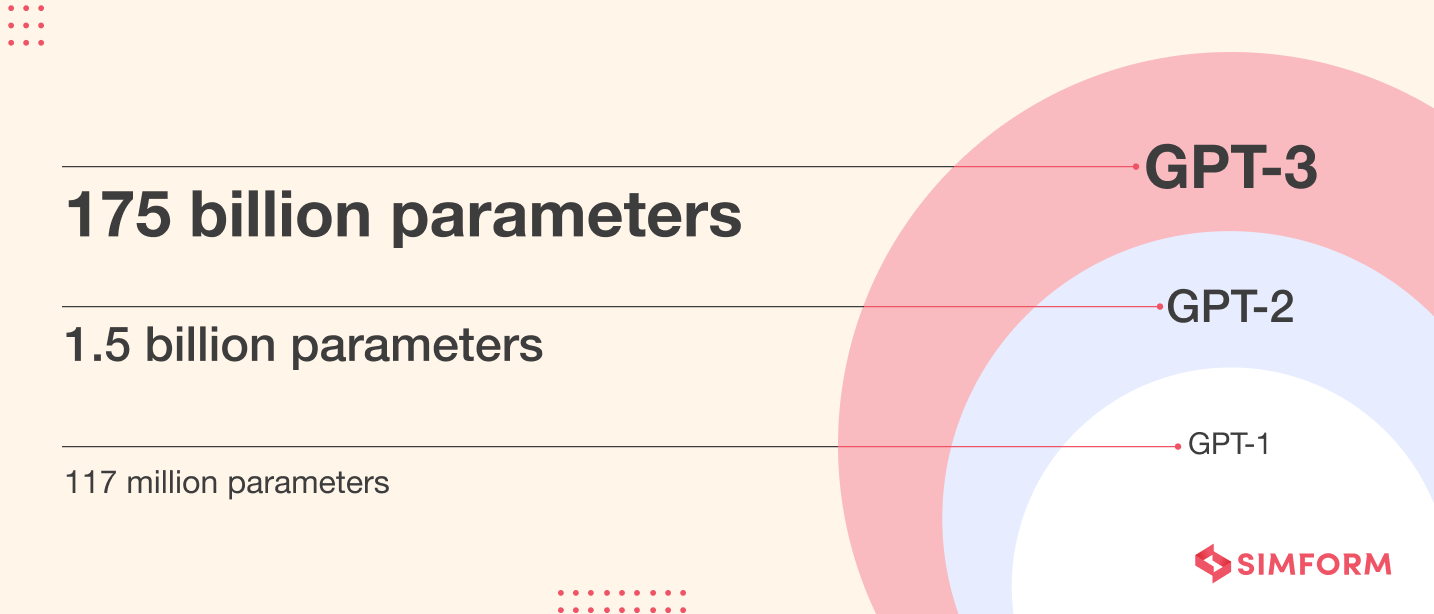
\includegraphics[scale=.55]{2-content/parameters-of-the-GPT-model.png}
    
    \caption{\url{https://www.simform.com/blog/the-gpt-model-comprehensive-guide/}}
    \end{figure}
\end{frame}

\begin{frame}[plain]{Wie funktioniert ein Sprachmodell}
    \begin{bee}[Aufgabe]
        Arbeite dich in 2er-Teams durch die Lernstrecke zu einfachen Textmodellen:
            \begin{enumerate}[1)]
                \item \url{https://inf-schule.de/ki/menueansicht/ki_erkunden/papagei/lernstrecke}
                \item Halte deine Erkenntnisse in schriftlicher Form fest.
            \end{enumerate}
    \end{bee} 
\end{frame}

\begin{frame}[plain,shrink=5]{KI Tools in der Radiologie}
    \begin{bee}[Aufgabe]
        Arbeitet in 5er-Gruppen und untersucht verschiedene online verfügbare KI-Tools aus der Radiologie.
        \begin{enumerate}[1.]
            \item Jede Gruppe untersucht \textbf{ein KI-Tool} aus der folgenden Liste:
            \begin{enumerate}[a)]
                \item \url{https://mlmed.org/tools/xray/}
                \item \url{https://ctread.com/x-ray}
                \item \url{https://maiahub.my}
                \item \url{https://image.galaxy.ai/ai-xray-analyzer}
                \item \url{https://www.medicai.io/free-tools/online-dicom-viewer}
            \end{enumerate}
            \item Diskutiert in eurer Gruppe folgende Fragen:
            \begin{enumerate}[a)]
                \item Was kann dieses KI-Tool analysieren?
                \item Welche Risiken oder Probleme könnten beim Einsatz entstehen?
            \end{enumerate}
            \item Präsentiert die Ergebnisse im Plenum
        \end{enumerate}
    \end{bee}
\end{frame}

%introduction-example
%\begin{frame}[plain]
%   \begingroup
%        \fontfamily{qag}\selectfont
%        \Huge\color{black}\textbf{Introduction}\\[0.6em]
%    \endgroup
%    \begingroup
%        Lorem ipsum dolor sit amet, consectetuer adipit
%    \endgroup
%\end{frame}


%real example
%\begin{frame}[plain]
%    \begin{bee}[Definición]
%        Sea $D$ un dominio de integridad. Una \textbf{\textit{función (o norma) euclídea}} sobre $D$ es cualquier función $v:D\backslash\{0\}\rightarrow\N$ tal que:
%            \begin{enumerate}[1)]
%                \item Para todo $a,b\in D$, con $a\neq 0$, existen $q,r\in D$ tal que $a=bq+r$, donde $r=0$ o $v(r)<v(b)$.
%                \item Para todo $a,b\in D$ no nulos, $v(a)\leq v(ab)$.
%            \end{enumerate}
%        Luego, un dominio de integridad $D$ es un \textbf{\textit{dominio euclídeo}} si existe una función euclídea en $D$.
%    \end{bee} 
%\end{frame}
